\begin{figure}[t]
\centering
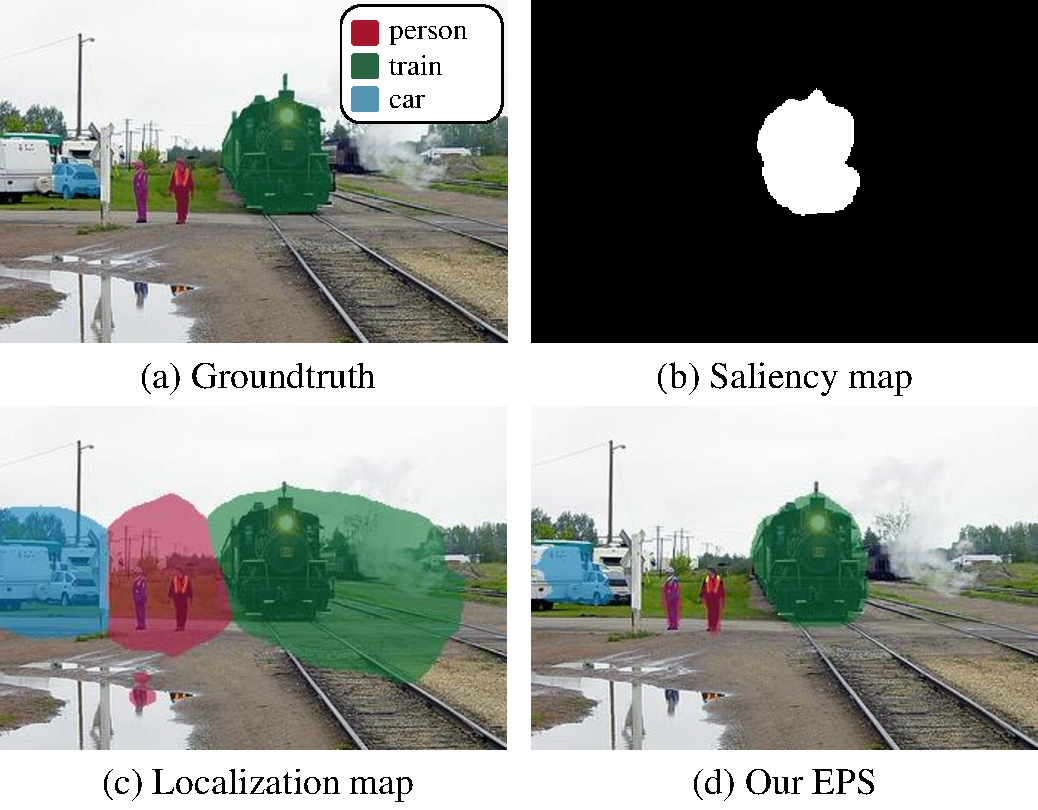
\includegraphics[width=8 cm]{figures/fig_concept.pdf}
\caption{WSSS를 위한 주목도 맵과 위치 맵을 모두 활용하는 동기 부여 예제. (a) 실제값, (b) PFAN~\cite{zhao2019pyramid}을 통한 주목도 맵, (c) CAM~\cite{zhou2016learning}을 통한 위치 맵, 그리고 (d) 분류기를 학습하기 위해 주목도 맵과 위치 맵을 모두 활용하는 우리의 EPS. 주목도 맵은 \emph{사람}과 \emph{자동차}를 포착할 수 없지만, 우리의 결과는 이를 올바르게 복원할 수 있으며, 위치 맵은 두 개의 객체를 과도하게 포착한다는 점에 유의하십시오.} \vspace{-2mm}
\label{fig:concept}
\end{figure}
